The study of neurodegenerative diseases such as Alzheimer's disease (AD) usually entails gathering different biomarkers of the disease coming from different sources \cite{Jack2010}: brain imaging techniques, cognitive assessments, or cerebrospinal fluid punctures. Over the past decades, such techniques have become widespread and there has been a surge in the number of available data. Large datasets from patients at different stages of the disease containing heterogeneous and over-time (longitudinal) data can help researchers in many ways: to gain insight on relationships between different biomarkers pointing to separate but dependent biologic processes; to stratify patients by stage or severity of the disease; to discover different subtypes or presentations of the disease for different groups of patients; or to improve disease prognosis (predicting its course). These applications could be of use in clinical trials by selecting relevant patients, thus increasing the power of the trial, or to quantify the evolution of subjects for better measuring the effect of treatment. For that, we need methods that can leverage and extract meaningful information from such complex data. \\

Machine learning (ML) is a set of techniques and models that have shown strong performance on a variety of tasks. These techniques are closely related to statistical methods and have gained a lot of popularity recently with the advent of deep learning (DL) \cite{LeCun2015}. ML techniques are relevant because of their ability in handling high dimensional data and extracting or discovering relevant patterns in it. ML techniques have been applied to medical data, including AD \cite{Litjens2017,Ching2018}. This is a field with many open challenges, and it will keep developing over the next years. An important challenge is to build methods that are able to find relationships between different biomarkers to improve our understanding of the progression of the disease. In this thesis, we explore machine learning and statistical methods that help us to gain insight on different aspects of AD using heterogeneous, longitudinal medical data. \\

\section{Alzheimer's disease}

% Severity of Alzheimer's Disease.
AD is, to date, an incurable neurodegenerative disease that causes a progressive degeneration of the brain and cognitive functions \cite{Lane2018}. Our current understanding is that the disease is characterized by an accumulation of amyloid-beta (A$\beta$) proteins in the brain and the formation of tau plaques, that leads to brain atrophy and gradually impair the cognition of the patients, who lose basic body functions like language or mobility, and finally leading to death, normally to external factors \cite{Ballard2011}. AD affects more than 47 million people worldwide, generating an estimated healthcare cost of around 604 billion US dollars a year \cite{AlzheimersAssociation}. As AD is a disease that generally affects elderly people, and accounting for the general aging of the population, this impact will only get stronger. It is estimated that, by 2030, 76 million people worldwide could be affected by this disease \cite{AlzheimersAssociation}. \\

Generally, when we talk about AD, we refer to sporadic late-onset AD, which has no known cause. There also exists a variant named autosomal dominant familial AD, affecting less than $5\%$ of AD patients \cite{Bird1993}, which is caused by genetic mutations in APP, PSEN1 and PSEN2 genes \cite{Campion1999}. It has an earlier age of onset, but it has a similar clinical presentation compared to its sporadic, most common form \cite{Ryan2016}. All work contained in this thesis is only applied to late-onset AD, and from now on it will be referenced in the text as AD for simplicity. \\

Up to present time, there has been no successful treatment to cure or slow down the cognitive decline caused by AD. Despite all the research on the topic, all clinical trials have failed \cite{Mehta2017} and did not manage to prove efficacy, even recent ones \cite{Huang2020}. Failures in drug design and development for AD could be linked to many reasons. One is that our understanding of the underlying processes that initially cause the cascade of events leading to the disease still needs to improve. Another reason could be that any potential successful drug would need to be administered at a presymptomatic stage of AD \cite{Mehta2017,Huang2020}. Detection of cognitively healthy patients at risk, or patients with very mild impairment that will progress to AD in the future is of utmost importance for future drugs and trials. \\ 

In the literature, diagnosis of patients is usually divided in three stages \cite{Brookmeyer2007}, although other classifications have been proposed \cite{Jack2018}:

\begin{enumerate}\itemsep5pt
\item Healthy control or cognitively normal (CN), when the patient shows neither signs of the disease nor cognitive problems.
\item Mild cognitive impairment (MCI), when the patient shows signs of cognitive impairment. It can be divided into two substages: early MCI and late MCI, differentiating between patients by their degree of cognitive impairment.
\item AD, when the patient is considered to have completely progressed into full-blown dementia.
\end{enumerate}

AD is a highly heterogeneous disease \cite{Lam2013}, meaning that symptoms and paths of neurodegeneration and cognitive decline can be different between groups of patients. Identifying different presentations or subtypes of the disease could help to improve detection of the disease and a better understanding of the interaction between different biological mechanisms and markers. In Chapter \ref{ch:3-cimlr} we present a method to identify subtypes of the disease. \\

AD has also been linked to several genetic mutation risks. Apart from the genes linked to the previously mentioned autosomal familial AD, the major genetic risk factor for AD is the Apolipoprotein E (APOE) $\varepsilon$4 allele \cite{Saunders1993}. It has been linked to an increased risk of AD, depending on the allele load \cite{Liu2013a} (if the patient has one or two copies of the allele). We study the APOE $\varepsilon$4 effect on hippocampal morphology of healthy patients at risk of AD in Chapter \ref{ch:5-pmhippocampus}.

\subsection{AD biomarkers}

To determine the current stage of the disease, various biomarkers describing the key pathophysiological processes of AD have been proposed over the years. AD is a multifactorial disease, with distinct progression paths depending on the observed biomarkers. AD is characterized by protein amyloid beta (A$\beta$) deposition in the brain \cite{Rissman2012}, tau injury, and structural neurodegeneration \cite{Jack2013}. Those three indicators precede cognitive impairment. For the measurement of these indicators, different biomarkers have been proposed:

\begin{enumerate}\itemsep5pt
\item Brain A$\beta$ deposition in the brain can be detected both in positron emission tomography (PET) imaging \cite{Clark2011}, and in cerebrospinal fluid (CSF) \cite{Andreasen1999}.
\item Tau injury and dysfunction caused by tau and p-tau plaques, found in tau-PET imaging and CSF \cite{Andreasen1999,Blennow2010}.
\item Neurodegeneration provoked by tau injury. It can be observed in structural magnetic resonance imaging (MRI) \cite{Weiner2005} and in fludeoxyglucose (FDG)-PET imaging \cite{Chetelat2003}.
\item Memory and cognition, measured by cognitive tests.
\end{enumerate}

The main screening tool for clinical assessment of AD is the clinical interview between the patient and the doctor, where the severity of the cognitive problems of the patient can be assessed, followed by a medical examination to capture the aforementioned biomarkers and assess the presence of the disease \cite{Lane2018}. \\

Imaging biomarkers for AD have are present in diagnostic criteria \cite{Lane2018} and have various advantages over other types of biomarkers. They can provide rich spatial information of the brain that cognitive assessments or amyloid levels cannot provide. They also have the potential to be sensitive at early stages of the disease, which allows us to study the early effects of the disease in the brain. We study the presymptomatic stage of AD in Chapter \ref{ch:5-pmhippocampus} using imaging biomarkers.  \\

Apart from the aforementioned biomarkers and imaging techniques, blood-based biomarkers have also been proposed for AD diagnosis \cite{Shi2018}, as they potentially could be a non-invasive, cheaper way to diagnose. Recently, plasma biomarker p-tau181 has shown promising results for an accurate AD diagnosis \cite{Karikari2020,Moscoso2020}. We use plasma biomarkers for our study in AD subtyping in Chapter \ref{ch:3-cimlr}. \\

\subsection{Longitudinal biomarker dynamics}

The previous biomarkers can be studied and modelled longitudinally. Modelling their trajectories and progression over time can give us more insight on how they change and interact. For example, longitudinal data analysis on MRI allows us to calculate the rate of change of specific brain structures, such as the dynamics of cortical and hippocampal atrophy. \\

A widely accepted progression model of AD was proposed by Jack et al. \cite{Jack2010}. Their model is based on biomarker evolution, where each biomarker progresses from normal values to abnormal values differently. The order of the biomarkers is presented above: A$\beta$ deposition, followed by tau injury, neurodegeneration, and cognition. Empirical data and experiments reviewed in \cite{Jack2013} confirm the validity of the model, although other data-driven works do not fully agree with it \cite{Iturria-Medina2016}. \\

%% Explicar aqui una mica de AD subtyping, del paper de young, tal tal
AD is a highly heterogeneous disease. It can overlap with other neurological pathologies and present different paths of neurodegeneration, with different rates of atrophy in different areas of the brain \cite{Lam2013,Poulakis2018}, distinct clinical and cognitive characteristics \cite{Murray2011} or even differences in other more specific biomarkers like CSF proteomics \cite{Tijms2020}. Development of methods to study the progression of AD should also take into account this heterogeneity for a better understanding of the disease. In Chapter \ref{ch:3-cimlr} we present a method for AD subtyping using blood-based biomarkers. \\

\section{Challenges in longitudinal and heterogeneous data}

Longitudinal data are composed of sequential data acquisitions for subjects over a period of time. This contrasts with cross-sectional studies, which focus on single acquisitions per subject. Here, we describe the main characteristics and analysis challenges that arise while dealing with longitudinal data. \\

Two sources of variability can be defined for a longitudinal study in a cohort of subjects: inter-subject variability, i.e. the differences between observations of different subjects, and intra-subject variability, i.e. the differences between observations of the same subject, which tend to be highly correlated compared to the former. Those two sources of variation give valuable information about the progression of the disease between- and within- subjects. In cross-sectional studies, those two variabilities are non-separable: given two samples of different subjects, it is not possible to know to what extent their variation is due to inter-subject variability or to the different stages of the disease. Adding longitudinal samples for each subject allows us to distinguish between those two variabilities, improving our understanding of the disease \cite{Fitzmaurice2008}. \\

\begin{figure}[htbp]
  \centering
  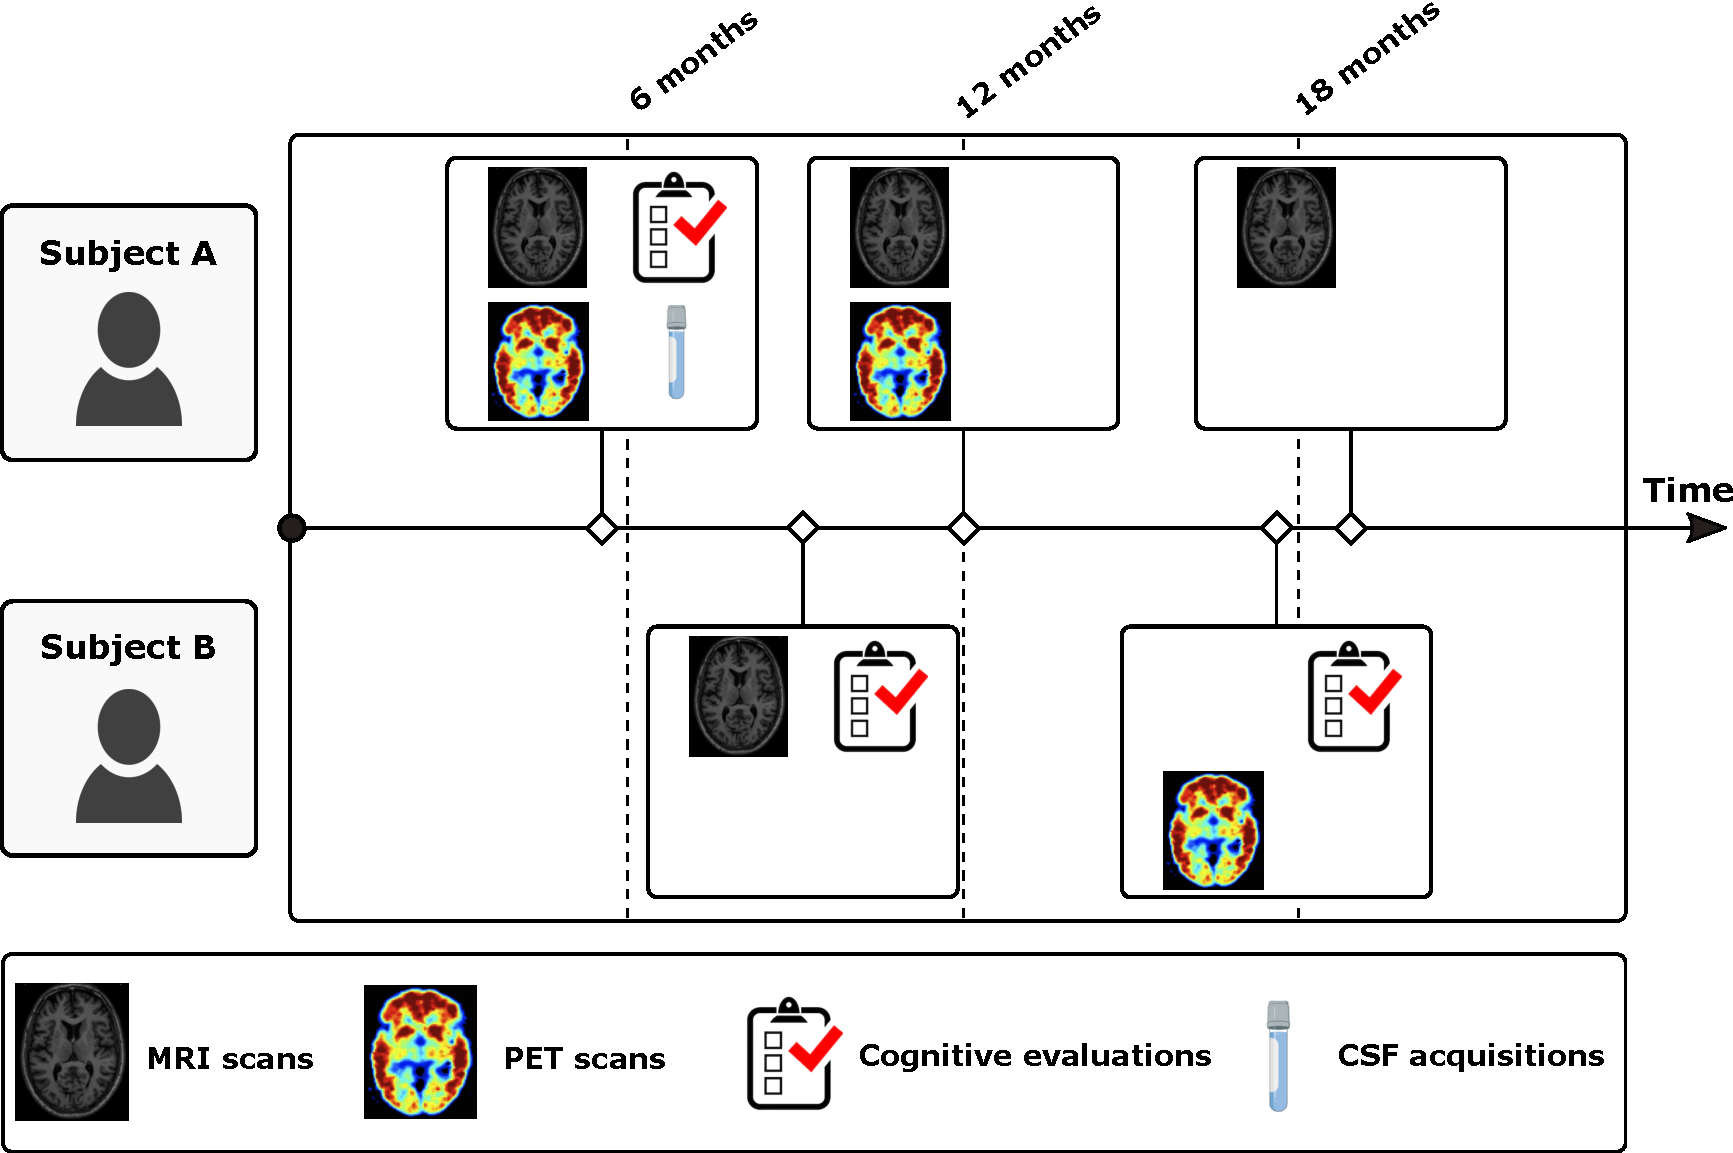
\includegraphics[width=0.9\textwidth]{figures/introduction/Fig-progression.pdf}
  \caption{Longitudinal representation of data acquisitions for two patients.}
  \label{long}
\end{figure}

Figure \ref{long} shows an example of a longitudinal study with two subjects, with multiple data modalities, over a fixed span of time. It illustrates some of the challenges that can appear in a longitudinal, multimodal data study: \\

\begin{enumerate}
\item Each subject can have a different number of acquisitions, leading to an unbalanced data problem. In the figure, Patient B only has one acquisition in the first year, compared to two for patient A.
\item There can be missing data due to missing acquisitions from some modalities. In the figure, only patient A at the 6-months follow-up has all the modalities.
\item Data are not necessarily acquired at the same time point for the different subjects.
\item Time spacing between follow-ups can be variable, even within a single subject.
\end{enumerate}

Another problem, not shown in the figure, is that different patients can be at different stages of the disease at a given time point. Reference time to measure progression remains an open issue in the field \cite{Ashford2001}.  \\

Protocols of data acquisition try to palliate these problems, but in a clinical setting, this is very difficult to achieve: sometimes patients miss their scheduled screening session and data cannot be gathered. Other patients might drop out from the study for a variety of reasons, such as disease severity or moving out of the city/country, and in other cases, data of a given time point could need to be discarded because of quality problems. For these reasons, most of the available longitudinal data is unbalanced. \\

\subsection{Studies and initiatives} 

There has been a remarkable number of initiatives to promote using longitudinal data on AD modelling. Availability of patients' longitudinal data is key to study the progression of the disease. Lawrence et al. \cite{Lawrence2017} presented a review of available longitudinal AD biomarker datasets, finding that more efforts are needed to increase the follow-up duration, increase the population size, and standardize the acquisition methods. One of the largest studies is the Alzheimer's Disease Neuroimaging Initiative (ADNI) \cite{Mueller2005}, a multimodal, ongoing longitudinal study with hundreds of enrolled subjects, gathering imaging data, cognitive scores, blood and CSF biomarkers. We use ADNI in Chapters \ref{ch:3-cimlr}, \ref{ch:4-rnnvae} and \ref{ch:5-pmhippocampus}. \\

Other studies focus on specific stages of the disease. The ALzheimer and FAmilies (ALFA) study \cite{Molinuevo2016} is a dataset of cognitively healthy subjects with a high proportion of subjects with one or two doses of APOE $\varepsilon4$, making the dataset ideal to study effects of AD at early stages and the possible effects of APOE $\varepsilon4$ in the preclinical phase of the disease. We use this dataset on Chapter \ref{ch:4-rnnvae} to study the hippocampus of cognitively healthy patients. \\

To unify and share the available data, the Alzheimer's Association created The Global Alzheimer’s Association Interactive Network (GAAIN)\footnote{\url{http://www.gaain.org}} to share data between independent studies and build collaborations to create and explore large, heterogeneous cohorts. More recently, a new initiative named Alzheimer's Disease Data Initiative (ADD)\footnote{\url{https://www.alzheimersdata.org/}} has been created for similar reasons of data unification and sharing. \\

\section{Machine learning for medical data}

Traditional methods for data analysis usually rely on searching relationships between measured quantities (e.g. variables). For example, in statistical inference, we start from a hypothesis of the effect of an independent variable on the dependent (output) variables, and look for relevant associations that confirm or refute the hypothesis. From another perspective, ML allows us to accurately model the relationship between input and output that generalize to unseen data. ML is particularly helpful when dealing with complex and unwieldy data, and when the number of input variables is large. Usually, ML models are trained for a specific task (e.g. image recognition or diagnosis prediction), but such techniques are also very useful to find patterns or relationships in high-dimensional data that could not be found otherwise due to the inherently complex nature of it. Lately, DL has become one of the most used ML tools for high-dimensional data. \\

ML has been applied to many healthcare problems. For example, breast cancer screening \cite{McKinney2020} or predicting cardiovascular risk factors on retina images \cite{Poplin2018}, have shown strong results using ML based techniques. A very prolific application of ML is medical imaging, where it has been used for image classification, segmentation, or synthetic data generation \cite{Litjens2017}. Use of such techniques also raises important technical and ethical questions, such as privacy concerns over data usage \cite{Yang2019} or bias or transparency issues \cite{Karikari2020, Haibe-Kains2020}. Nonetheless, the results achieved show their strength and potential for problems with high-dimensional, complex medical data. \\

ML has also been used in AD research for several tasks, such as diagnosis classification \cite{Rathore2017}, disease progression modelling \cite{Oxtoby2017} or disease subtpying \cite{Young2017}, to name a few. The inherent complexity between the different modalities of biomarkers of the disease and their temporal evolution and trajectories, coupled with the still unknown mechanisms underlying AD, make ML a prime candidate for the study of the disease. \\

\section{Contributions and outline of the thesis}

The main contributions of the thesis are presented in four main chapters, in addition to the introduction (Chapter \ref{ch:1-introduction}) and a final chapter with the general conclusions of our work (Chapter \ref{ch:6-conclusions}):

\begin{itemize}
    \item Chapter \ref{ch:2-review} reviews statistical and machine learning applications in AD using longitudinal neuroimaging. We perform a literature review of the field, selecting 105 papers to review. Our objective is to draw a clear picture of the state of the field, compare the current approaches and methods, and discover existing limitations. We show that methods that use longitudinal data have a strong potential for modelling disease progression and computer-aided diagnosis. 
    \item Chapter \ref{ch:3-cimlr} shows a study on AD subtyping using blood biomarkers. We apply an unsupervised clustering approach, based on multiple kernel learning, to study AD subtyping using novel plasma biomarkers. We obtain different subtypes of patients with different presentations of the disease, and we discover potential interactions between the groups using cross-sectional and longitudinal MRI based biomarkers.
    \item Chapter \ref{ch:4-rnnvae} presents a generative model based on variational autoencoders and recurrent neural networks that is able to combine multimodal longitudinal data with a variable number of time points. This method can predict the evolution of a given patient, show the relationships between modalities, and input missing channels. This is achieved by explicitly modelling the interdependencies between modalities and using recurrent neural networks to capture the evolution of each modality over time. We show the potential of the technique using synthetic and real data examples.
    \item Chapter \ref{ch:5-pmhippocampus} contains a study on the impact of APOE $\varepsilon$4 gene dose and its interaction with age on hippocampal shape, assessed with multivariate surface analysis, using an $\varepsilon$4-enriched cohort of cognitively unimpaired subjects. We discover relevant non-linear interactions that show how the hippocampus is affected in APOE $\varepsilon$4 subjects, and find similarities with the effect of AD on hippocampal shape using a second cohort containing patients at all stages of the disease.
\end{itemize}

These four chapters of the thesis are self-contained and adapted from peer-reviewed journal articles, or from articles in preparation (Chapter \ref{ch:4-rnnvae}). The citation to the original article can be found on the first page of each chapter. Supplementary files referenced to each subject can be found either on with the original journal article publication they are based from, or in the repository of the thesis\footnote{\url{https://github.com/GerardMJuan/PhD-Thesis-AD-ML}}.